% Fucking default pgfsys-dvipdfmx.def screws up normal text, so use another driver
%\def\pgfsysdriver{pgfsys-dvipdfm.def}
\documentclass[10pt, compress, protectframetitle, handout]{beamer}
% handout to deactivate \uncover
% usetitleprogressbar might be needed
%\usepackage{beamerprosper}

% Load BEFORE the theme
\usepackage{ulem}

\usetheme[progressbar=frametitle,block=fill]{metropolis}

\usepackage{pgfpages}
\usepackage{marvosym}
%\usepackage[marvosym]{tikzsymbols}
\usepackage{pgfplots}
\usepackage{tikz}
\usepackage{xifthen}
\usetikzlibrary{quotes,angles}
\usetikzlibrary{arrows}
\usetikzlibrary{calc,decorations.markings}
\usetikzlibrary{patterns}
\definecolor{myred}{rgb}{0.7,0.1,0.1}
\definecolor{myblue}{rgb}{0,0.447,0.741}
\definecolor{mygreen}{rgb}{0,0.498,0}
\definecolor{silvergray}{rgb}{0.752941176,0.752941176,0.752941176}
\setbeamertemplate{note page}[plain]
%\setbeameroption{show notes on second screen=right}

\usepackage{multirow}
\usepackage{multicol}
\usepackage{booktabs}
\usepackage{adjustbox}

\usepackage{datetime}
%	\usepackage[scale=2]{ccicons}
%	\usepackage{minted}
%	\usepgfplotslibrary{dateplot}
%	\usemintedstyle{trac}

\usepackage{textpos}
% Fixes bad positioning of hats
\usefonttheme{professionalfonts}%[onlymath]{serif}
\usepackage{subcaption}
%\usepackage{footmisc}
%\usepackage{epstopdf}
\usepackage{siunitx}
\usepackage{dcolumn}
\newcolumntype{d}[1]{D{.}{.}{#1}}
\DeclareSIUnit\atomicunit{a.u.}
\DeclareSIUnit\rydberg{Ry}
\usepackage{braket}
\usepackage{comment}
\usepackage{cancel}
%\includecomment{versionLONG}
\excludecomment{versionLONG}
\usepackage[sort&compress,square,semicolon]{natbib}

\def\qe{{\textsc Quantum ESPRESSO}}
\newcommand{\MATLAB}{MATLAB\textsuperscript{\textregistered}}


%%%%%%%%%%%%%%%%%%%%%%%%%%%%%%%%%%%%%%%%%%%%%%%%%%%%%%%%%%%
% datetime specific configuration                         %
%%%%%%%%%%%%%%%%%%%%%%%%%%%%%%%%%%%%%%%%%%%%%%%%%%%%%%%%%%%
\newdateformat{monthyear}{\monthname[\THEMONTH] \THEYEAR}

\graphicspath{{figures/PNG/}{figures/PDF/}{figures/}}

%\addtobeamertemplate{frametitle}{}{%
%\begin{textblock*}{1.5cm}(-0.7cm,0.7\textheight)
%\includegraphics[height=1.5cm]{logo_unitn}
%\end{textblock*}}

\title{Projection and Variational Monte Carlo simulations}
\subtitle{A presentation for the course in \emph{Computer Simulation}}
\date{May whenever, 2017}
\author{Matteo Seclì}
\institute{\scshape SISSA - Doctorate School in Condensed Matter
\vfill
\hfill
\includegraphics[height=1.3cm]{SISSA-LOGO.pdf}}
%\titlegraphic{\hfill
\includegraphics[height=1.3cm]{SISSA-LOGO.pdf}}

\addtobeamertemplate{frametitle}{}{%
\begin{textblock*}{100mm}(0.96\textwidth,-0.9cm)

\includegraphics[height=0.8cm]{sissa_logo_white.png}
\end{textblock*}}

\begin{document}

\maketitle

%\begin{frame}{Contents}
%	\tableofcontents
%\end{frame}


%\section{Introduction}
%
%\begin{frame}{Implementation choices}
%	
%	\begin{figure}
%		\centering
%		\includegraphics[height=0.25\textwidth]{Cpp_logo}
%		$\qquad$
%		\includegraphics[height=0.15\textwidth]{armadillo_logo}
%		$\qquad$
%		\includegraphics[height=0.25\textwidth]{QtCreator}
%		\bigskip\medskip\linebreak
%		\includegraphics[height=0.25\textwidth]{matlab_logo}
%		$\qquad\qquad$
%		\includegraphics[height=0.25\textwidth]{github_logo}
%	\end{figure}
%
%	Code at: \url{https://github.com/matteosecli/LJMC}.	
%	
%\end{frame}

\begin{frame}[standout]
	Code at:\\
	{\large \url{https://github.com/matteosecli/PMC-VMC}}
\end{frame}


\section{Projection Monte Carlo}

\begin{frame}{The system}

	Single particle in a 1D lattice with:
	\begin{itemize}
		\item $L$ sites
		\item A linear (site-dependent) potential $V(x) = V \cdot x$
		\item A hopping amplitude $t$
		\item Open boundary conditions
	\end{itemize}
	
	\begin{figure}
		\centering
		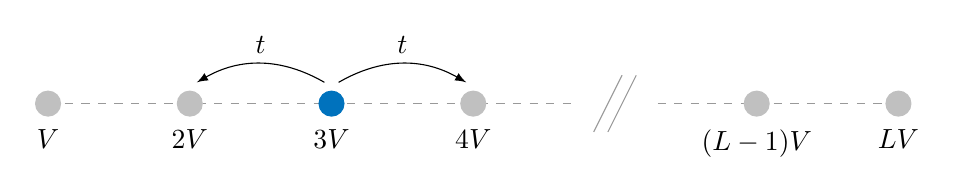
\begin{tikzpicture}[>=latex,transform shape,scale=1.0]
			\colorlet{TextColor}{.}
			\def\a{1.8}
			\def\Vlabel{0.6em}
			\draw[dashed,color=black!40!white,text=TextColor] (0,0) node[below=\Vlabel] {$V$} -- (1.0*\a,0) node[below=\Vlabel] {$2V$}  -- (2.0*\a,0) node[below=\Vlabel] {$3V$}  -- (3.0*\a,0) node[below=\Vlabel] {$4V$}  -- (3.7*\a,0);
			\draw[dashed,color=black!40!white,text=TextColor] (4.3*\a,0) -- (5*\a,0) node[below=\Vlabel] {$(L-1)V$} -- (6.0*\a,0) node[below=\Vlabel] {$LV$};
			\draw[color=black!40!white] (3.85*\a,-0.2*\a) -- (4.05*\a,+0.2*\a);% -- (4.1*\a,0);
			\draw[color=black!40!white] (3.95*\a,-0.2*\a) -- (4.15*\a,+0.2*\a);
			\draw[<-] (1.05*\a,0.15*\a) to[bend left] node[midway,above] {$t$} (1.95*\a,0.15*\a);
			\draw[->] (2.05*\a,0.15*\a) to[bend left] node[midway,above] {$t$} (2.95*\a,0.15*\a);
			\foreach \pos in {0,1,3,5,6}
			{
				\draw ({\pos*\a},0) node[circle,fill,color=silvergray] {};
			}
			\draw (2.0*\a,0) node[circle,fill,color=myblue] {};
		\end{tikzpicture}
	\end{figure}	
	
	\begin{equation}
		H = -t\sum_{\Braket{xx'}}c_{x'}^{\dagger}c_{x} + \sum_{x}V(x)c_{x}^{\dagger}c_{x}
	\end{equation}		
	
\end{frame}

\begin{frame}{Simulation results}

	\begin{figure}
		\centering
		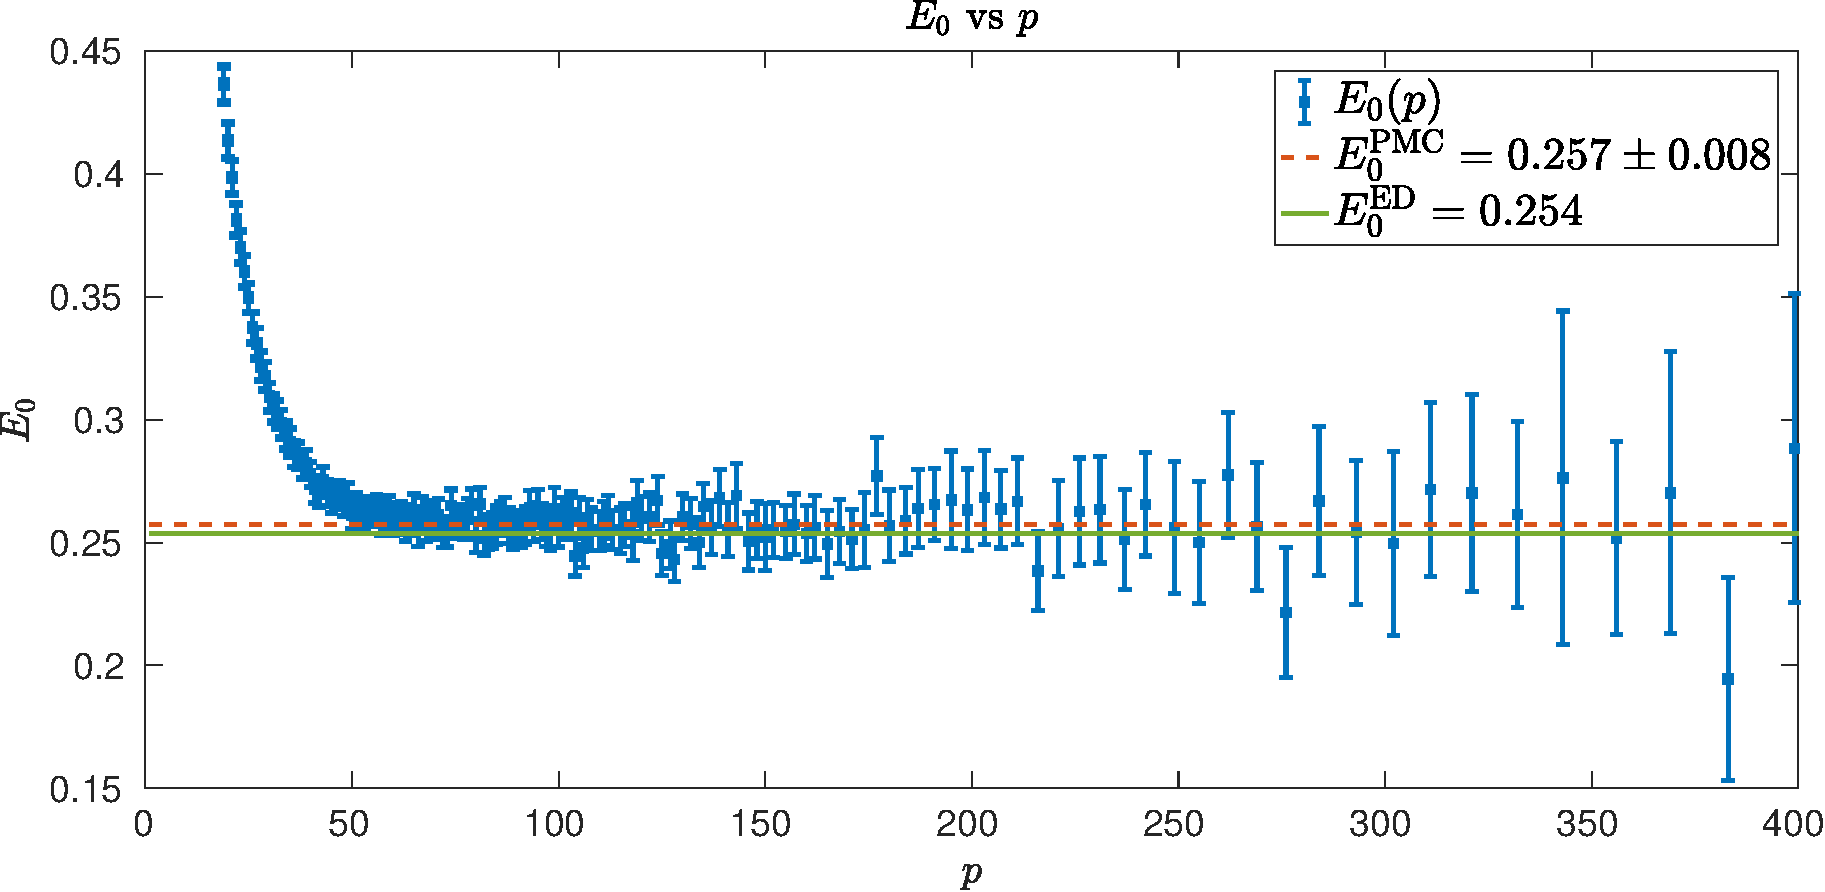
\includegraphics[width=\textwidth]{Evsp-10E7}
		\label{fig:Evsp-10E7}
		\caption{$E_0$ for $L=20$, $t=1$, $V=1$ and $N=10^7$. The mean position is $x_0 = 1.80 \pm 0.05$.}
	\end{figure}
	
\end{frame}

\begin{frame}{Simulation results}

	\begin{figure}
		\centering
		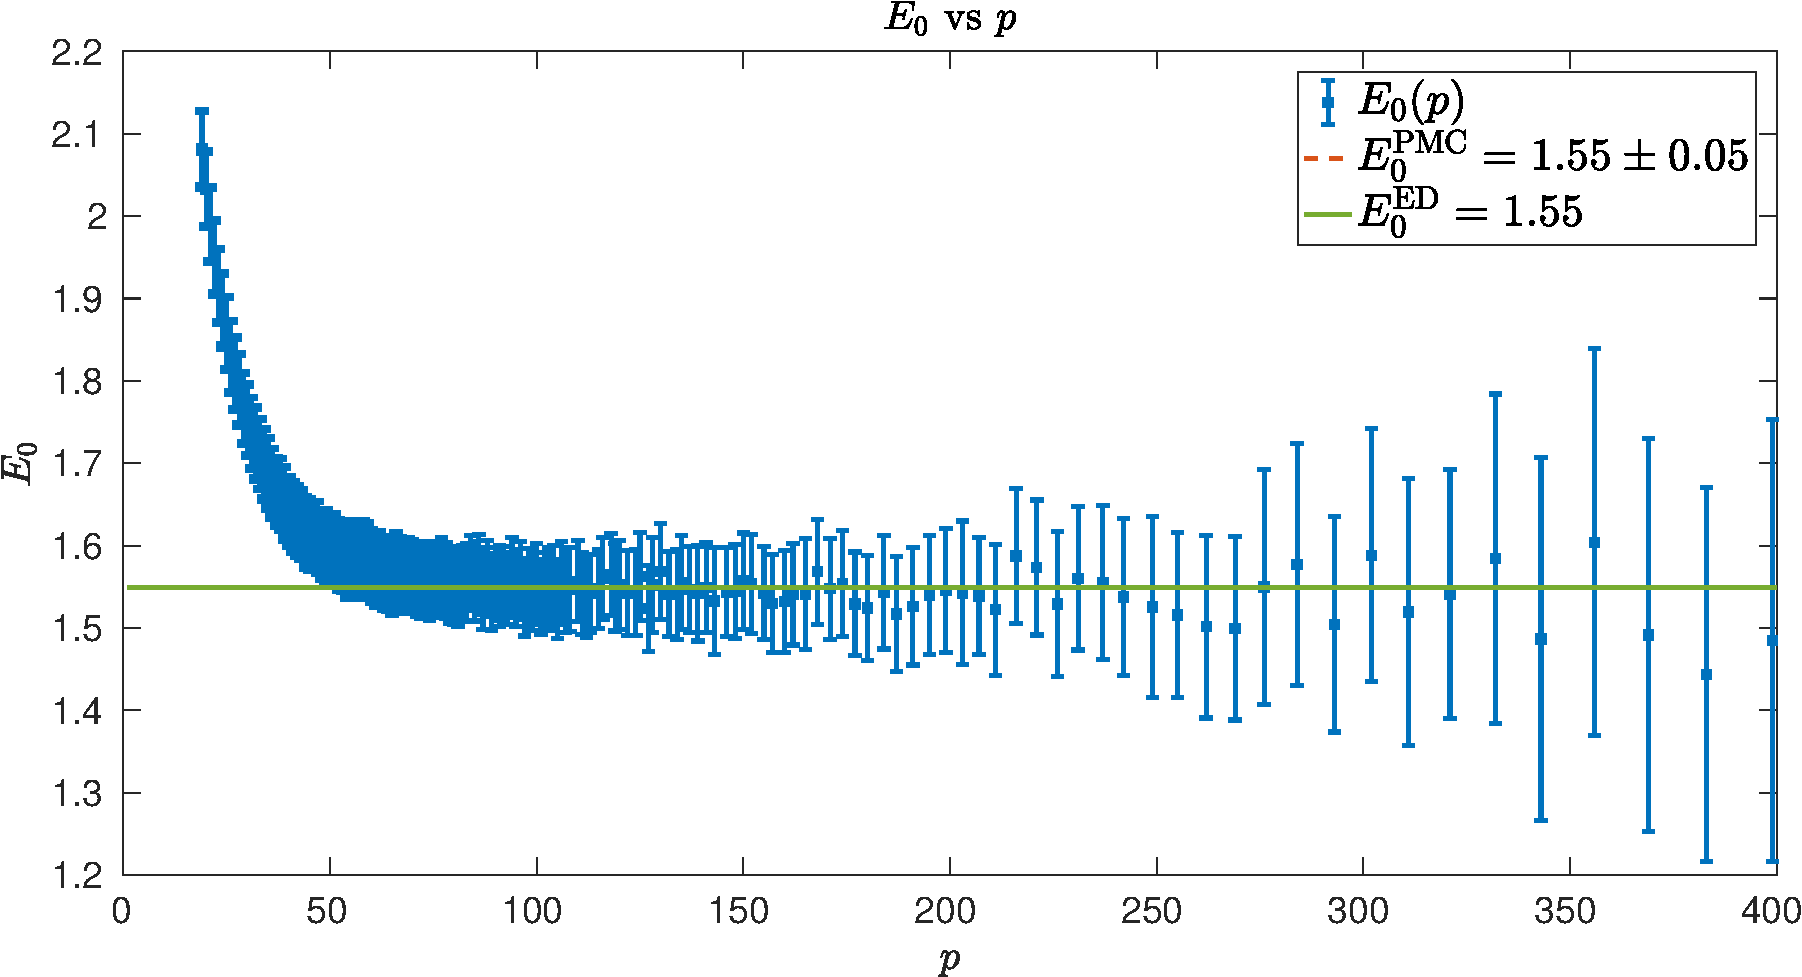
\includegraphics[width=\textwidth]{Evsp-10E7-V2}
		\label{fig:Evsp-10E7-V2}
		\caption{$E_0$ for $L=20$, $t=1$, $V=2$ and $N=10^7$. The mean position is $x_0 = 1.46 \pm 0.05$.}
	\end{figure}
	
\end{frame}

\begin{frame}{Simulation results}

	\begin{figure}
		\centering
		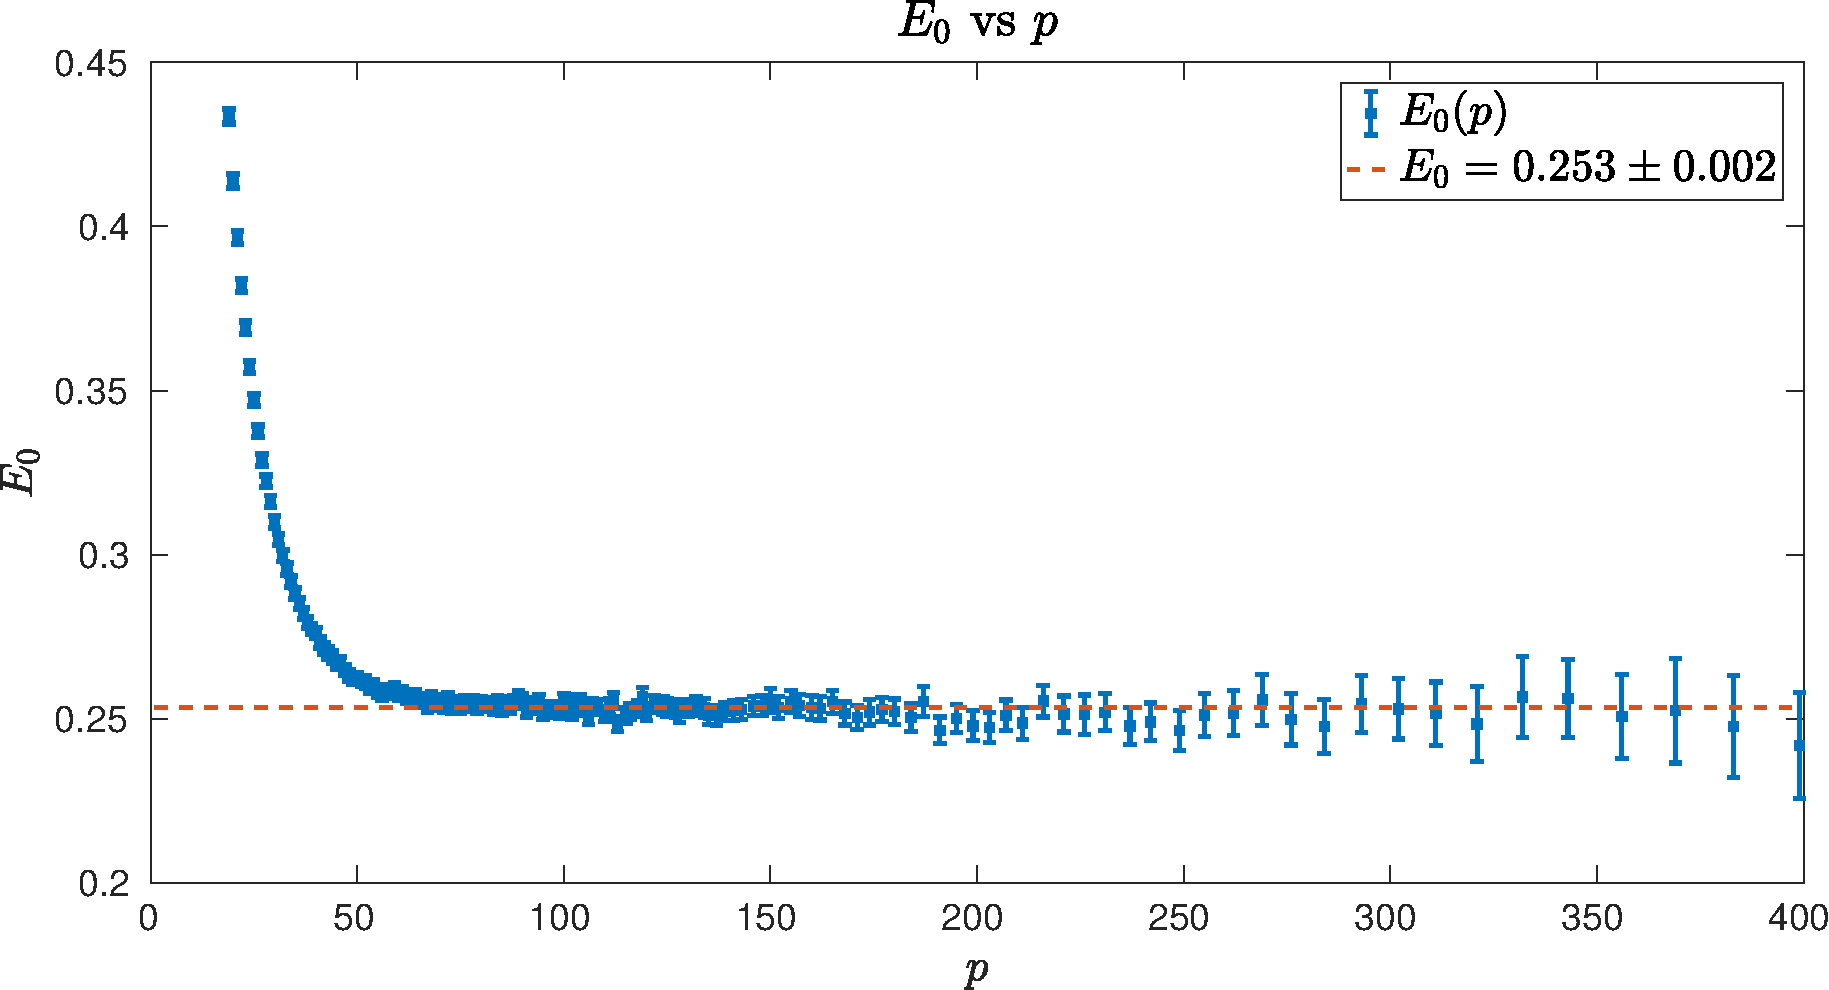
\includegraphics[width=\textwidth]{Evsp-10E8}
		\label{fig:Evsp-10E8}
		\caption{$E_0$ for $L=20$, $t=1$, $V=1$ and $N=10^8$. The mean position is $x_0 = 1.79 \pm 0.01$.}
	\end{figure}

\end{frame}
	
\begin{frame}{Simulation results}

	\begin{figure}
		\centering
		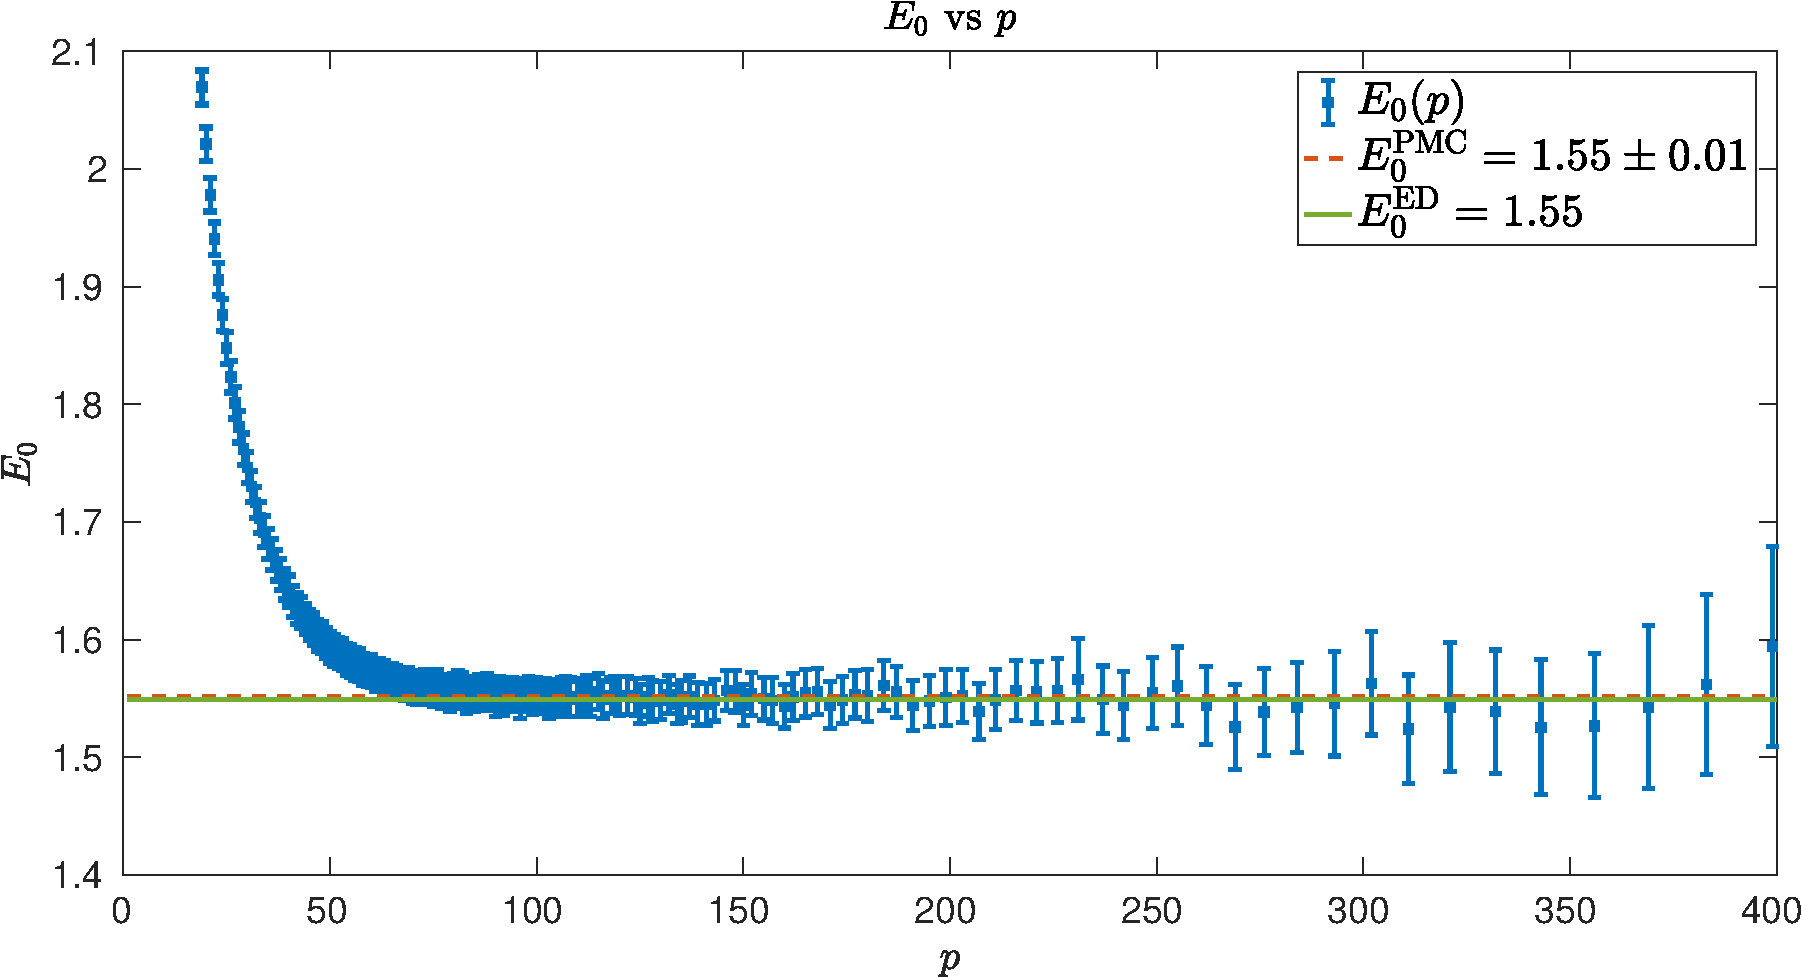
\includegraphics[width=\textwidth]{Evsp-10E8-V2}
		\label{fig:Evsp-10E8-V2}
		\caption{$E_0$ for $L=20$, $t=1$, $V=1$ and $N=10^8$. The mean position is $x_0 = 1.46 \pm 0.01$.}
	\end{figure}

\end{frame}



\section{Variational Monte Carlo}

\begin{frame}{The system}

	Antiferromagnetic spin-$1/2$ Heisenberg model on a 1D lattice with:
	\begin{itemize}
		\item $L$ sites
		\item Periodic boundary conditions
		\item Zero magnetization
	\end{itemize}
	
	\begin{figure}
		\centering
		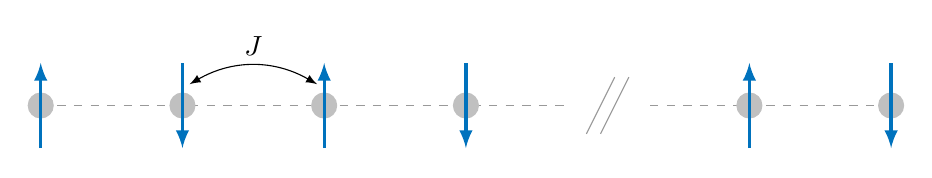
\begin{tikzpicture}[>=latex,transform shape,scale=1.0]
			\colorlet{TextColor}{.}
			\def\a{1.8}
			\def\Vlabel{0.6em}
			\draw[dashed,color=black!40!white,text=TextColor] (0,0) -- (1.0*\a,0) -- (2.0*\a,0) -- (3.0*\a,0) -- (3.7*\a,0);
			\draw[dashed,color=black!40!white,text=TextColor] (4.3*\a,0) -- (5*\a,0) -- (6.0*\a,0);
			\draw[color=black!40!white] (3.85*\a,-0.2*\a) -- (4.05*\a,+0.2*\a);% -- (4.1*\a,0);
			\draw[color=black!40!white] (3.95*\a,-0.2*\a) -- (4.15*\a,+0.2*\a);
			\draw[<->] (1.05*\a,0.15*\a) to[bend left] node[midway,above] {$J$} (1.95*\a,0.15*\a);
			\foreach \pos in {0,1,2,3,5,6}
			{
				\draw ({\pos*\a},0) node[circle,fill,color=silvergray] {};
			}
			\foreach \pos in {0,2,5}
			{
				\draw[->,very thick,color=myblue] ({\pos*\a},-0.3*\a) -- ({\pos*\a},+0.3*\a);
			}
			\foreach \pos in {1,3,6}
			{
				\draw[<-,very thick,color=myblue] ({\pos*\a},-0.3*\a) -- ({\pos*\a},+0.3*\a);
			}
		\end{tikzpicture}
	\end{figure}	
	
	\begin{equation}
		H 
		= J\sum_{i=1}^{L}\vec{S}_{i}\cdot\vec{S}_{i+1}
		= J\sum_{i=1}^{L}\left\lbrace
			S_{i}^{z}S_{i+1}^{z} + 
			\frac{1}{2}\left(S_{i}^{+}S_{i+1}^{-}+S_{i}^{-}S_{i+1}^{+}\right)
		\right\rbrace
	\end{equation}
	with $J>0$ in order to be antiferromagnetic.
	
\end{frame}

\begin{frame}[allowframebreaks]{The VMC procedure}

	\begin{itemize}
		\item Variational wavefunction on the basis of the configurations $\{\Ket{x}\}$ with definite $S_{i}^{z}$:
		\begin{equation}
			\psi(x) = \text{Sign}_{M}(x)e^{\frac{\alpha}{2}\sum_{i \neq j}v_{i,j}^{z}(2S_{i}^{z})(2S_{ij}^{z})}
		\end{equation}
		with $\text{Sign}_{M}(x) = (-1)^{\sum_{i=1}^{L/2}(S_{2i}^{z}+1/2)}$ and $v_{i,j}^{z} = 2\log(|2\sin(\pi(i-j)/L)|)$.
		\item Local energy:
		\begin{equation}
			E_L(x) = \frac{\Braket{x|H|\psi}}{\Braket{x|\psi}} 
			= \Braket{x|H|x} 
			+ \sum_{x' \neq x} \Braket{x|H|x'}\frac{\Braket{x'|\psi}}{\Braket{x|\psi}} 
		\end{equation}
		\item Staggered magnetization:
		\begin{equation}
			m = \Braket{ \left\lvert \frac{1}{L}\sum_{i=1}^{L}(-1)^iS_{i}^{z} \right\rvert }
		\end{equation}
		\item First neighbor correlation function:
		\begin{equation}
			C_1 = \Braket{\frac{1}{L}\sum_{i=1}^{L}S_{i}^{z}S_{i+1}^{z}}.
		\end{equation}
	\end{itemize}
	
	Exact results from Bethe ansatz in 1D\footnote{See Minoru Takahashi, \emph{Thermodynamics of One-Dimensional Solvable Models}. Cambridge University Press, 2005. ISBN 9780521019798.} ($L \to \infty$):
	\begin{equation*}
		E_{0} = -|J|\left(\log2-\frac{1}{4}\right) \simeq -0.4431471|J|
	\end{equation*}
	and
	\begin{equation*}
		C_1 = \frac{1}{12}\left(1-4\log2\right) \simeq -0.14771573.
	\end{equation*}
	
\end{frame}

\begin{frame}{Execution times}

	\begin{figure}
		\centering
		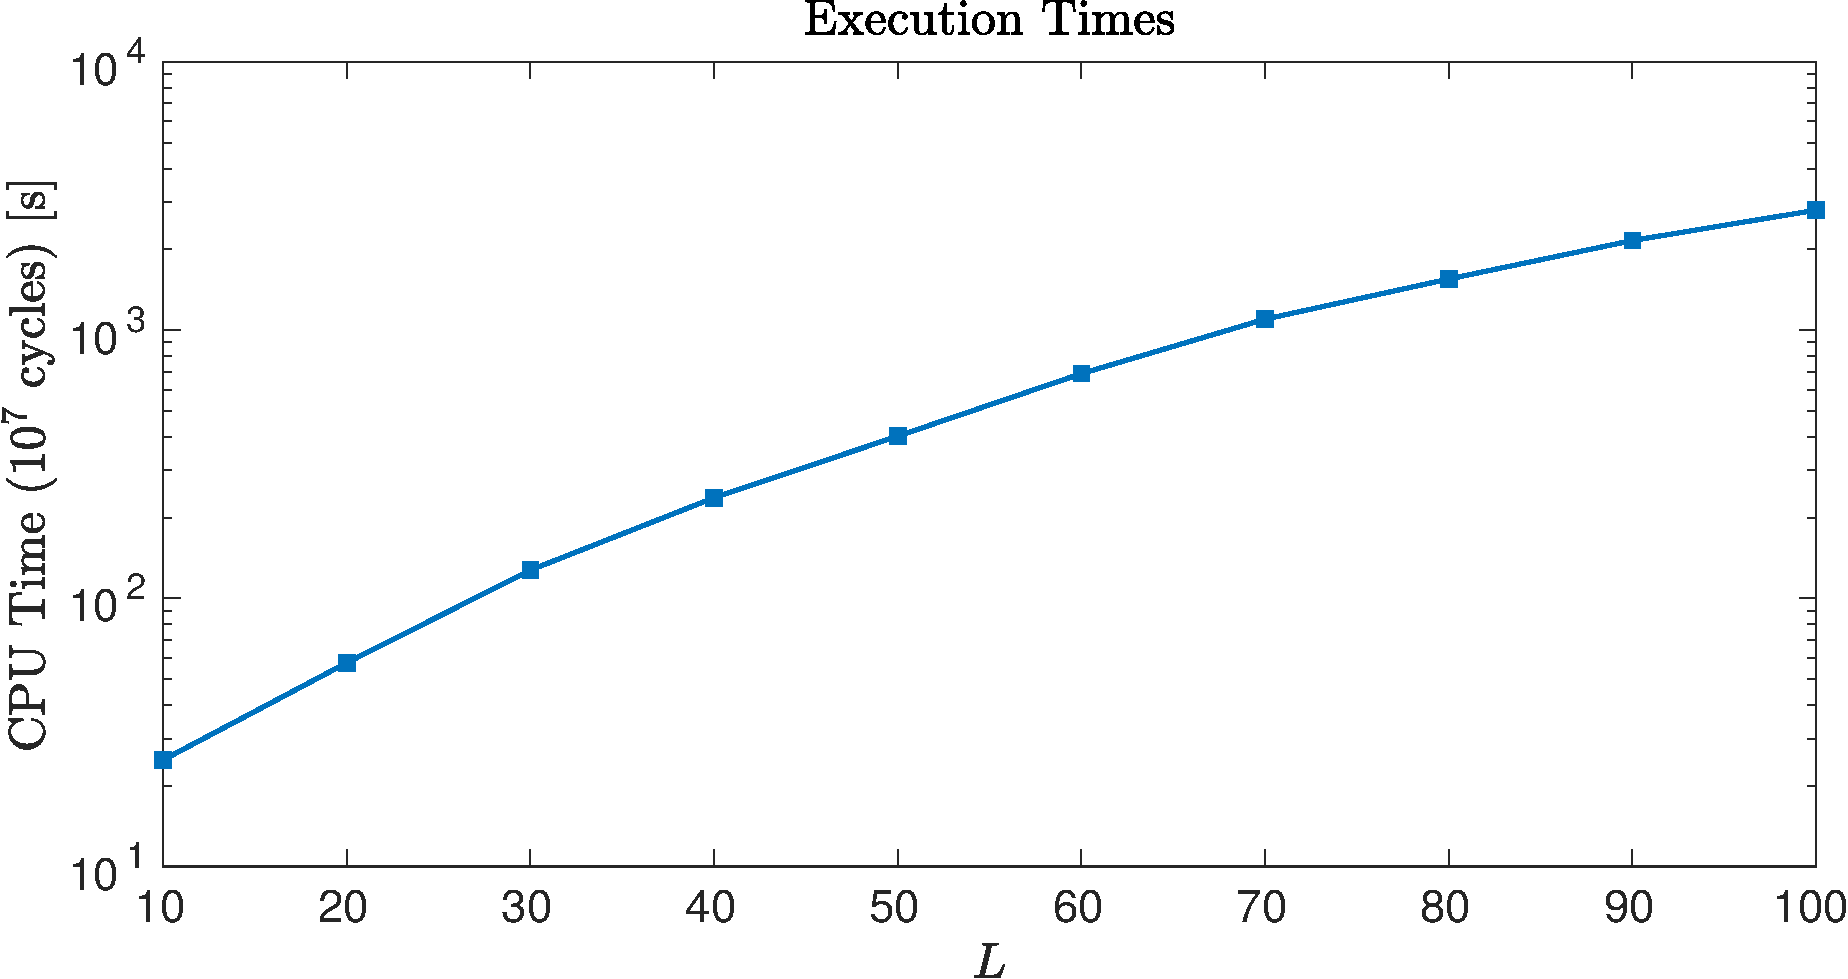
\includegraphics[width=\textwidth]{cputimes}
		\label{fig:cputimes}
		\caption{CPU time per variational parameter value with $10^7$ MC steps.}
	\end{figure}
	
\end{frame}

\begin{frame}{Simulation results}

	\begin{figure}
		\centering
		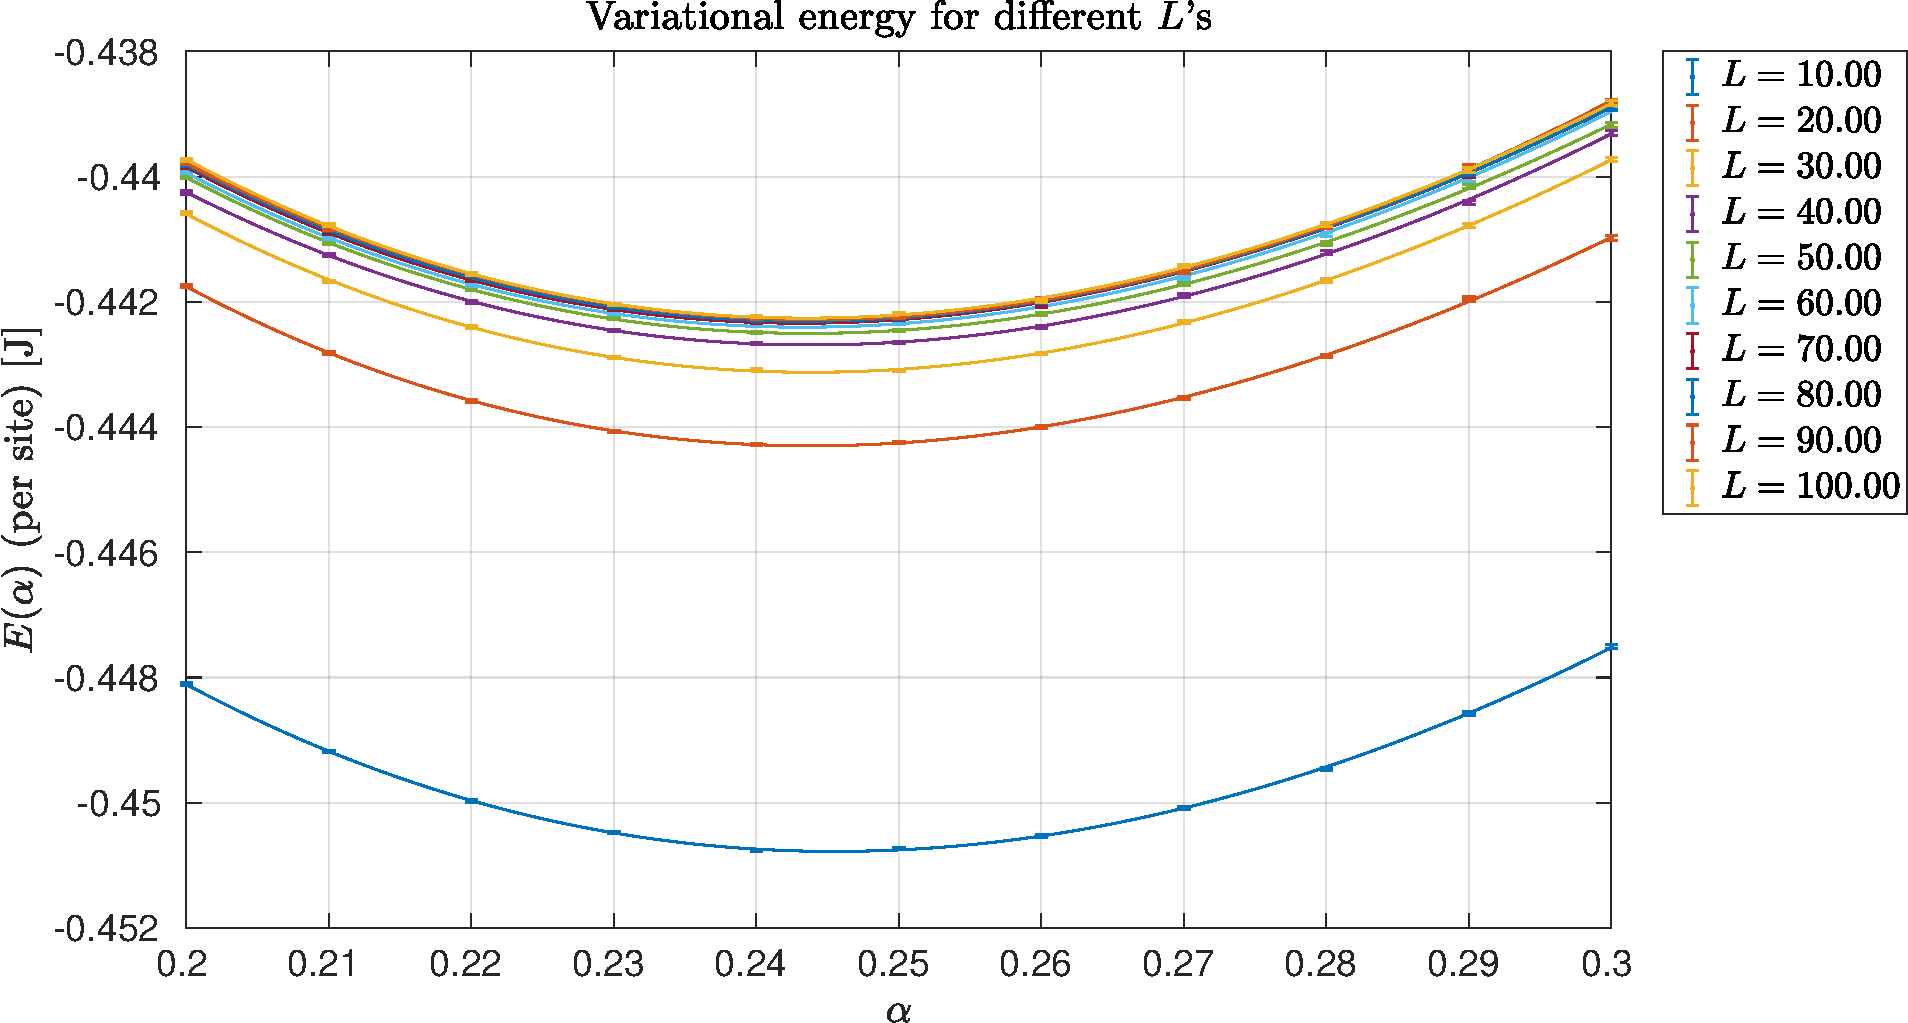
\includegraphics[width=\textwidth]{VariationalEnergies}
		\label{fig:VariationalEnergies}
		\caption{Variational energy. The best value for the variational parameter is estimated to be $\alpha = 0.244 \pm 0.001$.}
	\end{figure}
	
\end{frame}

\begin{frame}{Simulation results}

	\begin{figure}
		\centering
		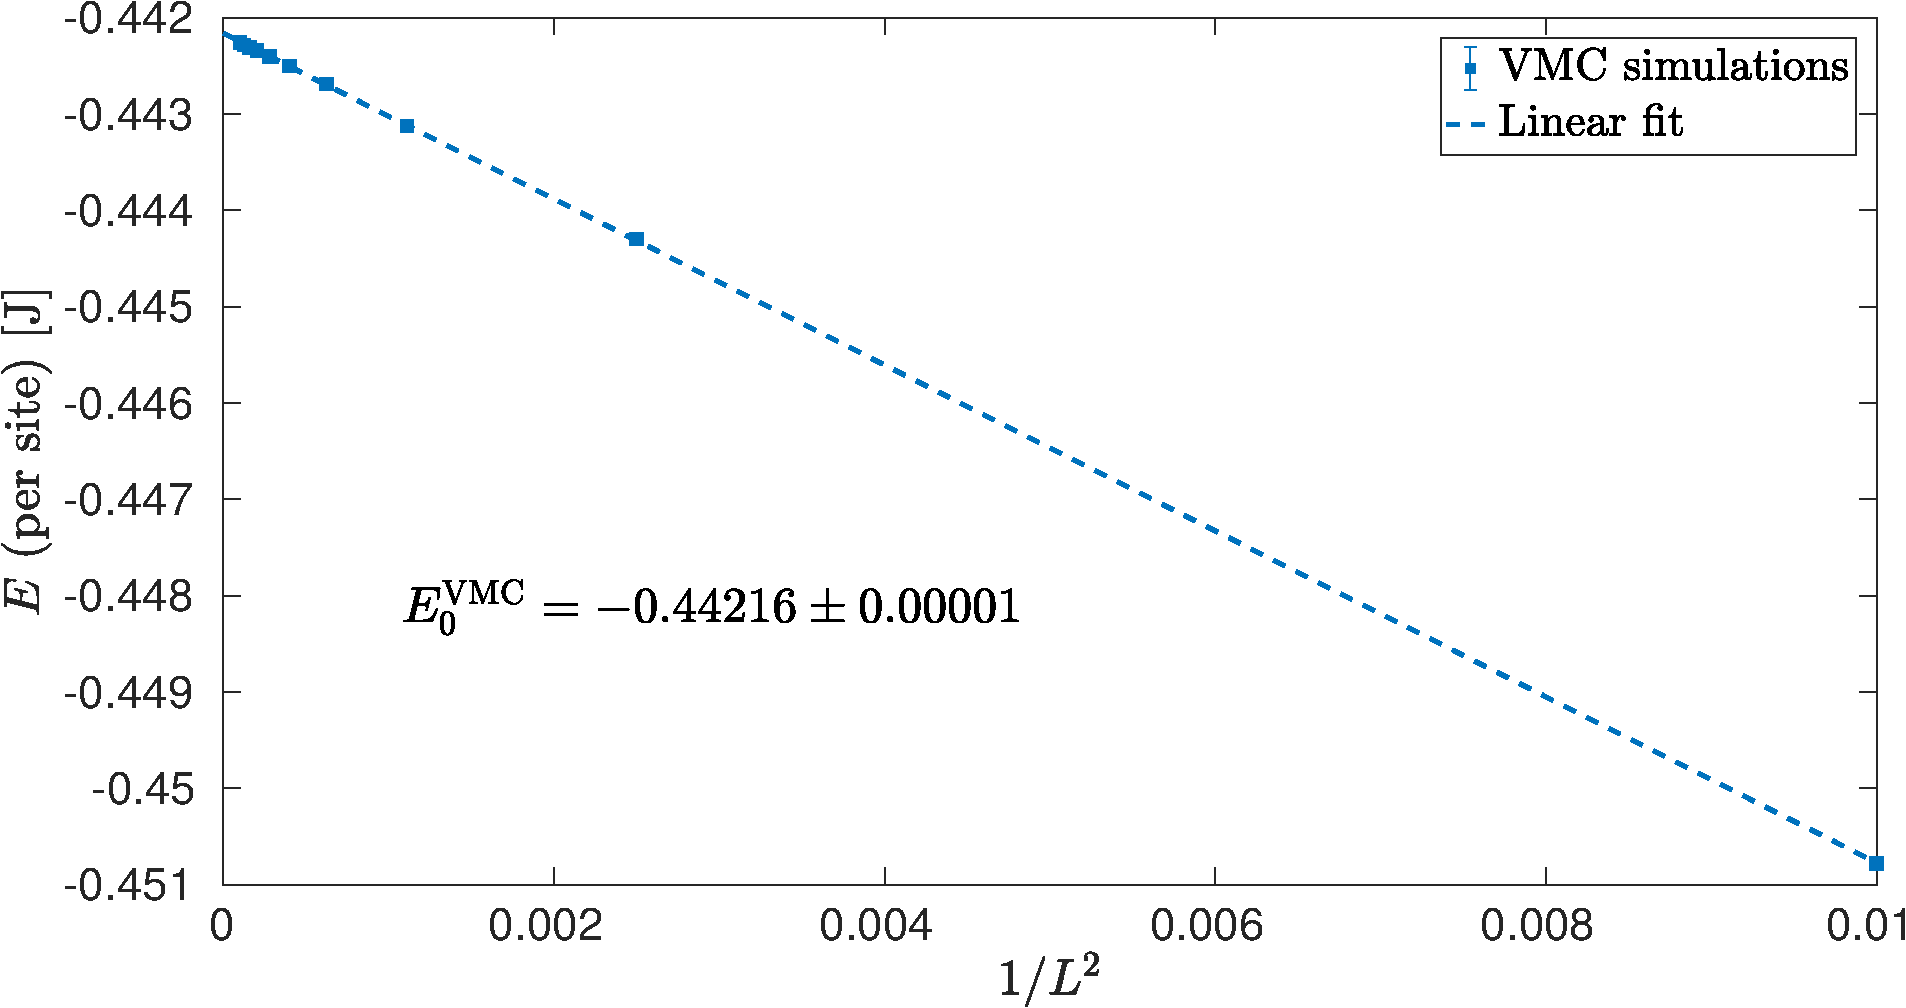
\includegraphics[width=\textwidth]{E_VMC}
		\label{fig:E_VMC}
		\caption{Extrapolation for $L \to \infty$.}
	\end{figure}
	
\end{frame}

\begin{frame}{Simulation results}

	\begin{figure}
		\centering
		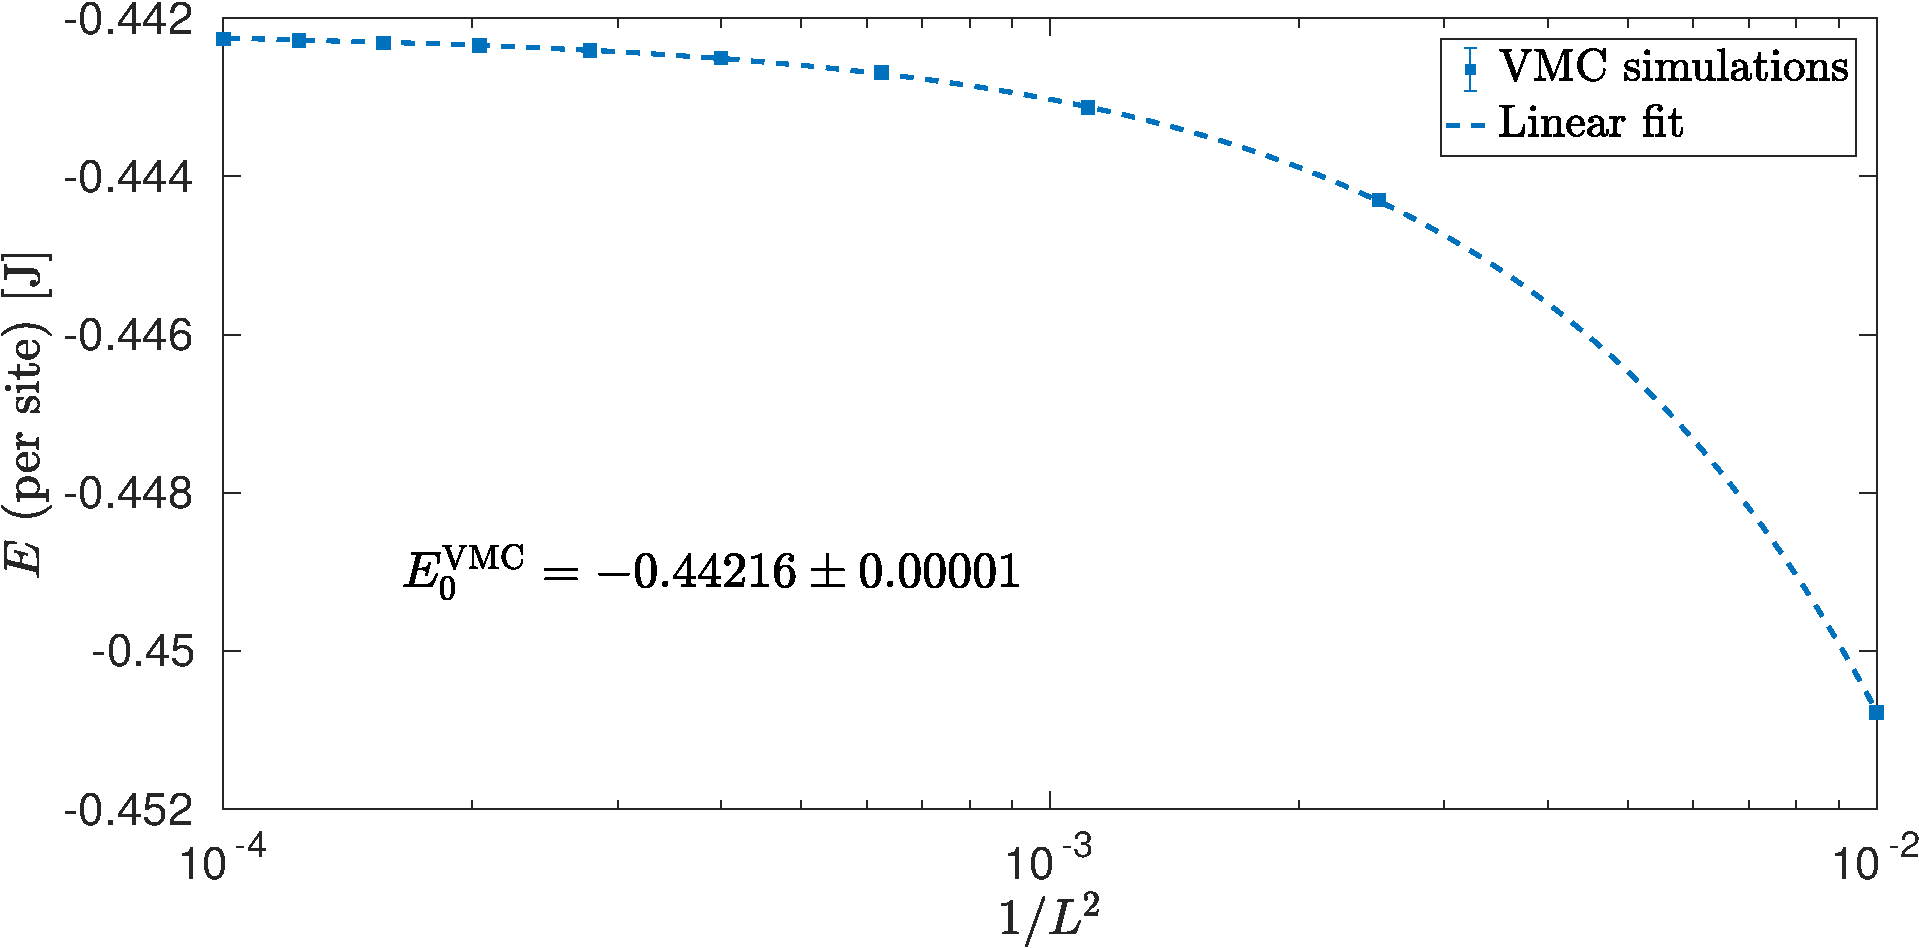
\includegraphics[width=\textwidth]{E_VMC_log}
		\label{fig:E_VMC_log}
		\caption{Extrapolation for $L \to \infty$.}
	\end{figure}
	
\end{frame}

\begin{frame}{Simulation results}

	\begin{figure}
		\centering
		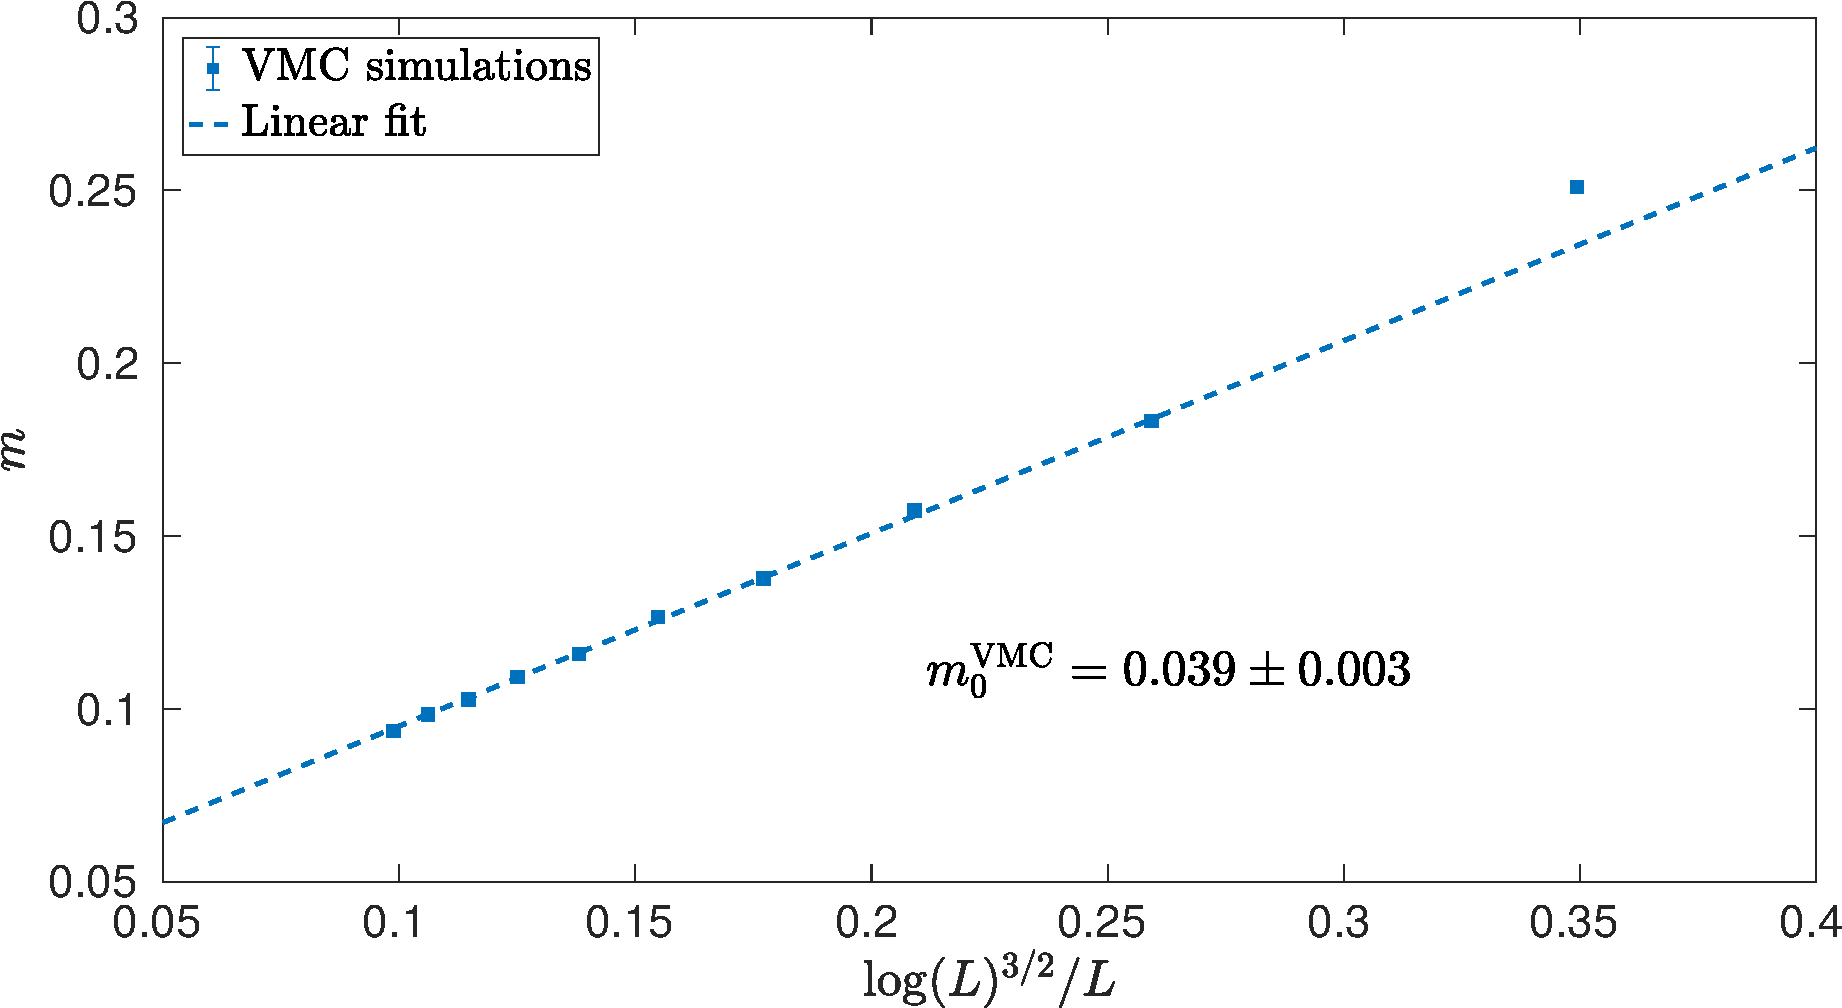
\includegraphics[width=\textwidth]{m_VMC}
		\label{fig:m_VMC}
		\caption{Extrapolation for $L \to \infty$.}
	\end{figure}
	
\end{frame}

\begin{frame}{Simulation results}

	\begin{figure}
		\centering
		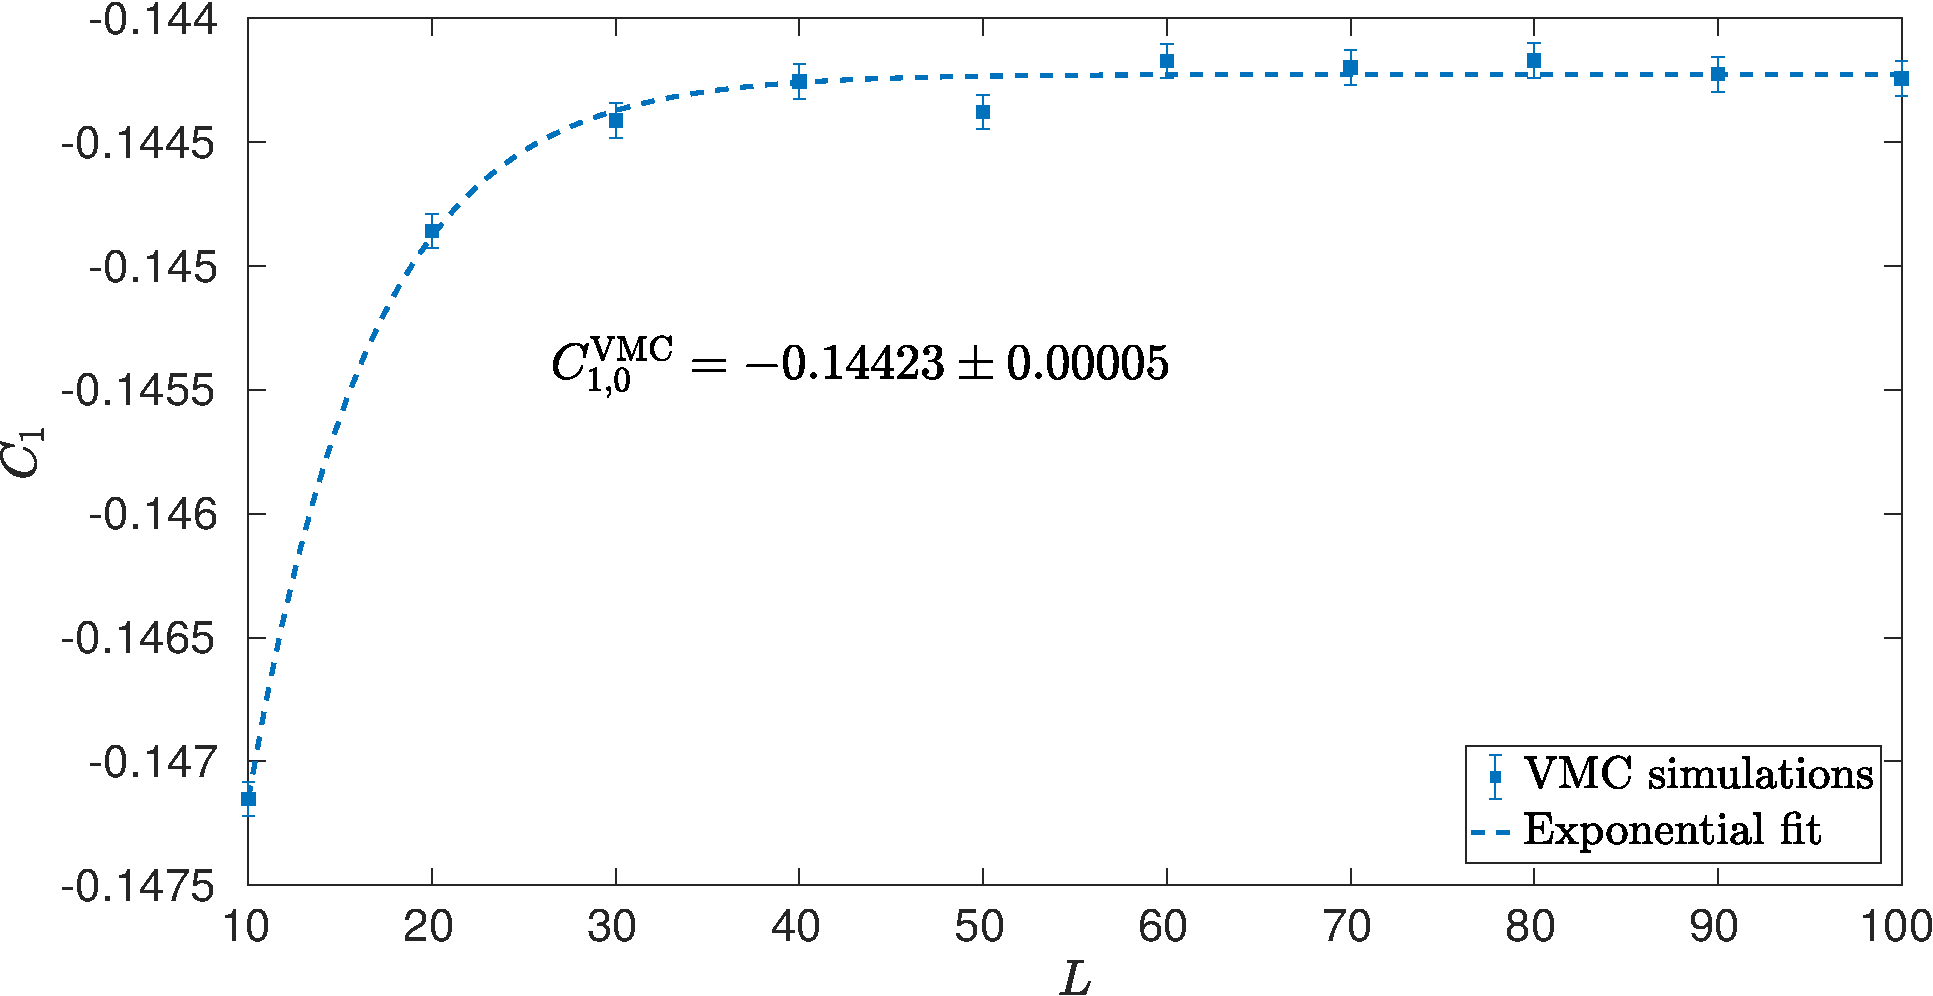
\includegraphics[width=\textwidth]{C1_VMC}
		\label{fig:C1_VMC}
		\caption{Extrapolation for $L \to \infty$.}
	\end{figure}
	
\end{frame}

\begin{frame}{Summary}

	\begin{table}[H]
	 	\begin{center}
	 		\begin{tabular}{lS[table-format=2.7]S[table-format=2.5]S[table-format=2.7]}
				\toprule
	 			{Method} & {$E_0$ [$J$]} & {$m$} & {$C_1$} \\
				\midrule
				Bethe ansatz\footnote{$L \to \infty$, exact.} & -0.443147 & 0 & -0.147716 \\
				VMC\footnote{$L \to \infty$, upper bound.} & -0.44216 \pm 0.00001 & 0.039 \pm 0.003 & -0.14423 \pm 0.00005 \\
				ED/Lanczos\footnotemark & -0.44304 \pm 0.00005 & {--} & {--} \\
	 			\bottomrule
	 		\end{tabular}
	 		\footnotetext{\label{ftn:giannozzi}Extrapolated to $L \to \infty$ from a set of calculations for $L=\{8,10,12,14,16\}$, with max $32$ steps for the Lanczos. Code: \url{http://www.fisica.uniud.it/~giannozz/Corsi/MQ/Software/C/heisenberg_exact.c}}
	 	\end{center}
	 	%\caption{Results for the 1D Heisenberg antiferromagnet with different methods.}
	 	\label{tab:results}
	\end{table}

\end{frame}


%\section{Conclusions}

\begin{frame}{Conclusions}

%	Just a brief summary of what we've done.
%
%	\begin{itemize}
%		\item BULLSHIT
%	\end{itemize}

	\uncover<+->{Hope this was at least a little bit interesting\ldots}
	
	\begin{center}
		\Large \uncover<+->{Thanks for your attention!}
		
		\Huge\uncover<+->{\Smiley}
	\end{center}

\end{frame}

\begin{frame}[standout]
	Questions?
\end{frame}

\begin{frame}[allowframebreaks]{References}

	\nocite{*}
	\bibliographystyle{plainnat}
	\bibliography{references/ref_database}

\end{frame}

\end{document}
